\chapter{\label{ch:pdj}Personagem do Jogador}

Este capítulo apresenta informações e demonstra como criar um Personagem do Jogador (PdJ). A seção~\ref{sec:PtosPdJ} explica a estrutura de pontos do PdJ e a seção~\ref{sec:fichaPdj} detalha os elementos da ficha, explicando um a um. Por fim, a seção~\ref{sec:criapdj} faz uma demonstração para criação de um personagem.

O RPG de Mesa terá dois tipos de personagens: 
\begin{itemize}
	\item Personagens do Mestre (PdM's ou NPC): Os PdM's são criados e controlados pelo narrador da mesa. A criação de PdM's é apresentada no Capítulo~\ref{ch:mestre} - \emph{Área do Mestre}.
	
	\item Personagem do Jogador (PdJ): O PdJ é criado e controlado por um dos jogadores da mesa. Cada jogador controla pelo menos um personagem.
\end{itemize}

Antes de começar a preencher a ficha, é preciso que o jogador faça um breve planejamento de como será o personagem que deseja interpretar na aventura. Sugerimos que o jogador escreva em uma folha de caderno (tipo rascunho) uma pequena descrição do personagem que deseja construir,


\section{\label{sec:PtosPdJ}Pontos de personagem}

No Sistema +2d6@ifsul, um personagem é inicialmente representado por uma descrição textual que é ``convertida'' para pontos de atributos, perícias, vantagens e desvantagens. Esses pontos serão registrados na ficha de personagem, que é uma representação numérica do PdJ.

Quanto maior a pontuação registrada na ficha, mais poderoso é o personagem naquele aspecto. Entretanto, o jogador não pode registrar a pontuação que quiser nos atributos, pois isto deixaria o personagem ``invencível'', de forma que o jogador precisa ``comprar'' as características que deseja com uma quantidade limitada de pontos.

O Mestre da aventura determina quantos pontos estarão disponíveis para ``compra'' de características, enquanto os jogadores precisam escolher em quais aspectos pretendem ``investir'' em seu personagem, com os pontos disponíveis.

A pontuação apresentada na Tabela~\ref{tblPtos} é uma sugestão conforme o tipo de aventura:

\begin{table}[htb]
	\centering\smaller
	\caption{Quantidade de Pontos por tipo de aventura.}
	\begin{tabularx}{\textwidth}{|X|X|X|}
		\hline
		&	\multicolumn{2}{c|}{\textbf{Tipo de aventura}} \\
		\hline
		\textbf{Aspecto}	&	\textbf{Heroicas ou Fantasia} &	\textbf{Realista ou Horror} \\
		\hline
		Para Atributos		& 20 a 25 pontos  	& 10 a 15 pontos	\\
		\hline
		Para Perícias		& 15 pontos  				& 10 pontos\\
		\hline
		Para Vantagens		& 5 pontos mais pontos obtidos com desvantagens 				& apenas pontos obtidos com desvantagens \\
		\hline
		Obtidos com Desvantagens	& obter até 5 pontos  	& obter até 5 pontos \\
		\hline
	\end{tabularx}
	\label{tblPtos}
\end{table}

A definição desta pontuação vai depender de como será a aventura. Se por exemplo o Mestre construir uma onde os personagens sejam muito fortes, poderia estabelecer 30 pontos para atributos, 25 para perícias e 15 para vantagens mais 10 para vantagens obtidos com desvantagens.

Para as aventuras baseadas neste Livro de Regras, a pontuação para atributos será limitada entre 1 e 5. Atributos com pontos acima de 5 representam personagens com capacidades sobre-humanas, enquanto atributos com 0 pontos representam incapacidade total. 

Aventuras com personagens sobre-humanos precisam de ajustes não abordados neste livro de regras\footnote{Para saber mais sobre os níveis sobre-humanos, consulte a versão completa do Sistema +2d6 no site do autor \url{https://newtonrocha.wordpress.com/sistema-de-rpg-2d6/}}. 

\section{\label{sec:fichaPdj}Ficha de personagem}
A ficha de personagem é o local onde são mantidas as informações do PdJ. Os atributos, perícias, vantagens e desvantagens são representados por pontos (valores numéricos). A Figura~\ref{fichaMaoLivre} mostra uma Ficha de Personagem exemplo, que pode ser feita a mão livre em uma folha de caderno. Outros modelos são mostrados no Apêndice~\ref{apendiceFichas}.

Os principais elementos da Ficha de Personagem são: 
\begin{itemize}
	\item ATRIBUTOS: Representam as capacidades físicas e mentais do personagem. Ver seção~\ref{subsecAtributos}.
	\item PERÍCIAS: São habilidades/ofícios aprendidas/conquistadas pelo personagem antes da aventura, no seu passado. Ver seção~\ref{subsecPericias}.
	\item VANTAGENS e DESVANTAGENS: São características/poderes que afetam o personagem. Vantagens auxiliam/ajudam em determinadas situações, enquanto desvantagens prejudicam/atrapalham.  Ver seção~\ref{subsecVantagens}.
\end{itemize}

 
\begin{figure}[htb]
	\centering\smaller
	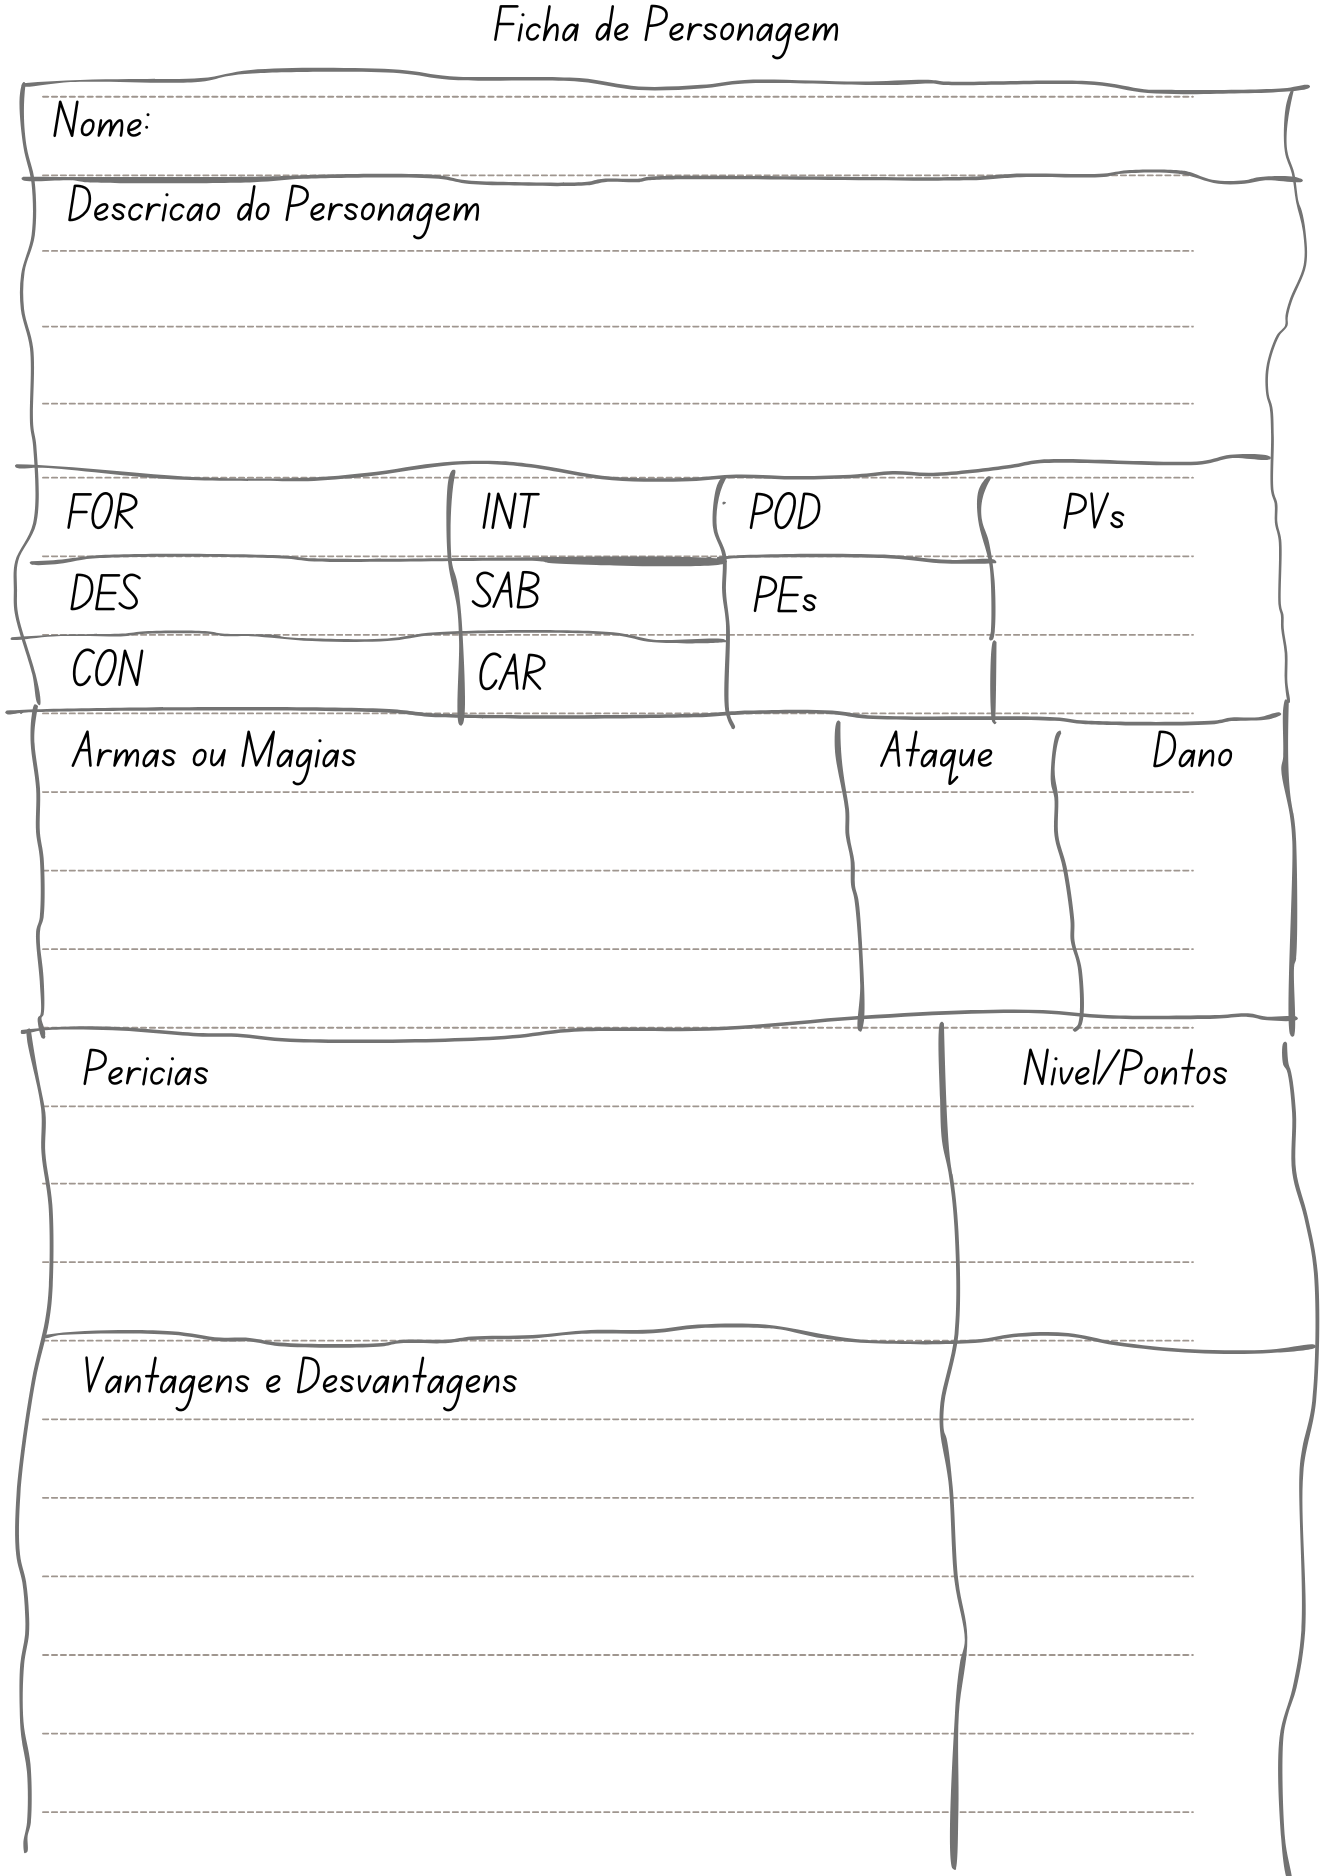
\includegraphics[scale=0.9]{img/fichaManual2.png}
	\caption{Exemplo de ficha feita a mão livre.}
	\label{fichaMaoLivre}
\end{figure}


\subsection{\label{subsecAtributos}Atributos}
Os atributos usados para definir/quantificar as características básicas de um personagem. Na criação do PdJ, o jogador ``investe'' uma quantidade de pontos em cada atributo, dando forma ao seu personagem.

Os atributos são organizados da seguinte forma:
\begin{itemize}
	\item \textbf{Físicos}: FORÇA, DESTREZA e CONSTITUIÇÃO.
	\item \textbf{Mentais}: INTELIGÊNCIA, SABEDORIA e CARISMA.
	\item \textbf{Mágicos, sobrenaturais, cibernéticos ou outros}: PODER.
\end{itemize}

Como pode ser verificado na ficha de personagem, o PdJ também têm Pontos de Vida, Redução de Dano e Pontos de Energia. Os Pontos de Vida serão definidos juntamente com a Constituição enquanto Pontos de Energia e Redução de Dano são definidos em seções específicas.

\subsubsection*{Força (FOR)}

Pontuação que representa a força física do personagem. É um atributo importante (requer maior pontuação) para personagens focados em ação física como guerreiros, lutadores marciais, soldados, gladiadores, paladinos, templários, etc.

FOR é necessária para o PdJ executar ações que precisam de força como levantar carros, entortar barras de ferro, usar espadas e lanças, defender-se de feras selvagens, entre outros. Também é usada no cálculo dos Pontos de Vida (PV) do personagem (ver Tabela~\ref{tbl:pvInicial}).

A Tabela~\ref{tbl:forca} faz uma descrição da capacidade para a pontuação da força e do Dano causado por ataques ``a mão livre'' (como luta de boxe, por exemplo). O valor de Dano pode ser acrescentados ao dano da arma corpo-a-corpo (ver seção~\ref{sec:combate}), desde que todos os jogadores da mesa estejam de acordo.

\begin{table}[htb]
	\centering\smaller
	\caption{Pontuação em força.}
	\begin{tabu} to 0.85\textwidth {|X[c ]|X[c]|X[c 2]|} \tabucline-
		\textbf{Força} 	& \textbf{Dano a mão livre} & \textbf{Capacidade equivalente} \\ \tabucline-		
		1 & 1d6-3 	&	Levanta uma cadeira \\ \tabucline-
		2 & 1d6-1 	&	Levanta uma mesa \\ \tabucline-
		3 & 1d6		& 	Levanta um peso de 100kg \\ \tabucline-
		4 & 1d6+1	&	Levanta um peso de 200kg\\ \tabucline-
		5 & 1d6+2	&	Levanta um peso de 400kg\\ \tabucline-
	\end{tabu}
	\label{tbl:forca}
\end{table}


\subsubsection*{Destreza (DES)} 

Pontuação que representa a agilidade, reflexos, pontaria e equilíbrio do personagem. É um atributo importante (requer maior pontuação) para personagens focados agilidade como ranger, monges, guerreiros, ladinos, ninjas, etc.

DES é necessária para ações que precisam de agilidade como escalar paredes/muros, esquivar dos golpes de espada, esquivar do bote de um animal peçonhento, entre outros. Personagens com valores pontuação elevada em destreza, recebem \emph{bônus em testes de esquiva e ataques a distância} (coluna Bônus), conforme mostrado na Tabela~\ref{tbl:destreza}.

\begin{table}[htb]
	\centering\smaller
	\caption{Pontuação em destreza.}
	\begin{tabu} to 0.85\textwidth {|X[c]|X[c]|X[c 2]|} \tabucline-
		\textbf{Destreza} 	& \textbf{Bônus} 	& \textbf{Capacidade} \\ \tabucline-		
		1 					& sem  								& Sedentário	\\ \tabucline-
		2 					& sem 								& Faz exercícios regulares	\\ \tabucline-
		3 					& +1 de bônus. 						& Acrobata amador \\ \tabucline-
		4 					& +2 de bônus. 						& Acrobata profissional \\ \tabucline-
		5 					& +3 de bônus. 						& Ninja\\ \tabucline-
	\end{tabu}
	\label{tbl:destreza}
\end{table}

\subsubsection*{Constituição (CON)}
Pontuação que representa a vitalidade, folego, resistência a doenças ou venenos de um personagem. É um atributo importante (requer maior pontuação) para personagens focados em combate como bárbaros, paladinos, etc.

CON é necessário para testar se o personagem resistiu a algo, como ao veneno de um animal peçonhento, a uma determinada doença, se consegue ficar embaixo da água prendendo a respiração, entre outros. 

Os pontuação de constituição também impacta diretamente na quantidade de Pontos de Vida (PV) do personagem. Além disso, personagens com pontuações elevadas em constituição normalmente recebem pontos de vida extra. A Tabela~\ref{tbl:const} faz uma descrição da capacidade para a pontuação da força e mostra a quantidade de pontos de vida extra.

\begin{table}[htb]
	\centering\smaller
	\caption{Pontuação em constituição.}
	\begin{tabu} to 0.85\textwidth{|X[c]|X[c]|X[2c]|} \hline
		\textbf{Constituição}	& \textbf{PV Extra} &	\textbf{Capacidade}  \\ \tabucline-
		\hline
		1		& 0 		& Sedentário, cansa rapidamente (15 min correndo).	\\ \tabucline-
		2		& 1  		& Corpo normal, cansa com esforço físico moderado (30 min correndo). 		\\ \tabucline-
		3		& 3 		& Corpo de atleta amador, cansa após esforço físico forte. (1h correndo). 	\\ \tabucline-
		4		& 5   		& Corpo de atleta profissional, cansa após esforço físico pesado (4h correndo). 		\\ \tabucline-
		5		& 7 	  	& Corpo de atleta campeão olímpico, cansa após esforço físico muito pesado (8h correndo). 	\\ \tabucline-
	\end{tabu}
	\label{tbl:const}
\end{table}

\subsubsubsection*{Pontos de Vida Iniciais} 
Os Pontos de Vida (PV) iniciais do personagem são definidos já na sua criação. A Tabela~\ref{tbl:pvInicial} faz duas sugestões para o cálculo dos PV iniciais, conforme o tipo de aventura e incluindo os pontos de vida extra por constituição ($pvExtra$, obtido na coluna PV Extra da Tabela~\ref{tbl:const}).

\begin{table}[htb]
	\centering\smaller
	\caption{Cálculo para Pontos de Vida Inicial}
	\begin{tabu} to 0.75\textwidth{|X[c]|X[2c]|X[2c]|} \hline
		&				\multicolumn{2}{c|}{\textbf{Tipo de aventura }} \\ \tabucline-
		\textbf{Constituição}	 &	\textbf{Heroicas / Fantasia} &	\textbf{Realistas / Horror} \\ \tabucline-
		1		&  $20+CON+FOR+pvExtra+1d6$ 	& $10+CON+FOR+pvExtra+1d6$	\\ \tabucline-
		2		&  $20+CON+FOR+pvExtra+1d6$ 	& $10+CON+FOR+pvExtra+1d6$	\\ \tabucline-
		3		&  $20+CON+FOR+pvExtra+1d6$ 	& $10+CON+FOR+pvExtra+1d6$	\\ \tabucline-
		4		&  $20+CON+FOR+pvExtra+2d6$ 	& $10+CON+FOR+pvExtra+2d6$	\\ \tabucline-
		5		&  $20+CON+FOR+pvExtra+2d6$ 	& $10+CON+FOR+pvExtra+2d6$	\\ \tabucline-
	\end{tabu}
	\label{tbl:pvInicial}
\end{table}

\subsubsection*{Inteligência (INT)}
Pontuação que representa a capacidade de raciocínio e memória do personagem. É um atributo importante (requer maior pontuação) para personagens focados em atividades que exijam raciocínio e memória como magos, hackers, investigadores, etc.

INT é necessária para ações que precisam de raciocínio e memória, como conhecer e conjurar magias arcanas, compreender um pergaminho, lembrar de uma informação que estava em um livro da biblioteca, conhecer outros idiomas, criar um vírus, etc. A Tabela~\ref{tbl:inteligencia} apresenta uma descrição da capacidade dessa pontuação.

\begin{table}[htb]
	\centering\smaller
	\caption{Pontuação em inteligência.}
	\begin{tabu} to 0.85\textwidth{|X[c]|X[2c]|} \hline
		\textbf{Inteligência}	 &	\textbf{Capacidade}  \\ \tabucline-
		\hline
		1		 		& Inteligência normal.	\\ \tabucline-
		2		  		& Inteligência acima da média. 		\\ \tabucline-
		3		 		& Inteligência muito acima da média. 	\\ \tabucline-
		4		   		& Gênio 		\\ \tabucline-
		5		 	  	& Super gênio. 	\\ \tabucline-
	\end{tabu}
	\label{tbl:inteligencia}
\end{table}


\subsubsubsection*{Idiomas conhecidos (Regra opcional)}
Uma aventura pode ser ambientada em um universo ficcional com vários idiomas. Neste caso, pode ser interessante adotar uma regra para idiomas conhecidos. 

Um personagem muito inteligente certamente vai conhecer (ou tem mais chances de aprender) mais idiomas do que os companheiros ``com inteligência menor''. Esta regra pode ser adotada para, por exemplo, testar se um personagem consegue ``ler'' um antigo pergaminho em língua desconhecida até então.

A Tabela~\ref{tbl:idiomas} faz uma sugestão para controle da quantidade de idiomas conhecidos, conforme a inteligência do PdJ. Observe que o conhecimento linguístico em aventuras ambientadas no tempo medieval\footnote{Fato histórico: Na Idade Média, saber ler e escrever era privilégio de poucos. Este conhecimento era restrito aos nobres e ao clero, ou seja, o povo (plebeus) não tinha acesso e nem mesmo permissão para aprender a ler.} é bem precário quando comparado com aventuras em universos modernos. A tabela também diferencia saber ler e escrever. 

\begin{table}[htb]
	\centering\smaller
	\caption{Idiomas conhecidos segundo inteligência.}
	\begin{tabu} to \textwidth{|X[c]|X[c]|X[c]|X[c]|X[c]|} \tabucline-
						&	\multicolumn{2}{c|}{\textbf{Universo Medieval}} & \multicolumn{2}{c|}{\textbf{Universo Moderno}} \\ \tabucline-
	\textbf{Inteligência}	& Sabe ler 		&	Sabe escrever 		&	Sabe ler 		&	Sabe escrever 			\\ \tabucline-
		1				&	Nativo			& não					& 	Nativo			& Nativo 					\\ \tabucline-
		2				&	Nativo			& Nativo				& 	Nativo + 1  	& Nativo + 1  \\ \tabucline-
		3				&	Nativo + 1 		& Nativo  				& 	Nativo + 2 		& Nativo + 2  \\ \tabucline- 		
		4				&	Nativo + 2 		& Nativo + 1 			& 	Nativo + 4 		& Nativo + 4  \\ \tabucline-	
		5				&	Nativo + 3 		& Nativo + 2 			& 	\multicolumn{2}{c|}{Poliglota}	\\ \tabucline-
	\end{tabu}
	\label{tbl:idiomas}
\end{table}

A lista de idiomas disponíveis no universo precisa ser definida pelo Mestre.

\subsubsection*{Sabedoria (SAB)}
Pontuação que representa a capacidade de percepção, intuição, sensibilidade e conhecimento intuitivo de um personagem. É um atributo importante (requer maior pontuação) para personagens tipo clérigo, druida, médium, naturalistas, rangers, monges, etc.

SAB é necessária em ações como reconhecer se uma planta é ou não venenosa, perceber se um povoado está sendo receptivo a sua visita, para conectar-se com algum deus ou força da natureza, intuir perigo, perceber motivação, energias místicas ou presenças sobrenaturais, entre outros. 

Personagens com valores pontuação elevada em sabedoria, recebem \emph{bônus em testes de intuição e força de vontade}. A Tabela~\ref{tbl:sabedoria} faz uma sugestão para valores de bônus por sabedoria.

\begin{table}[htb]
	\centering\smaller
	\caption{Pontuação em constituição.}
	\begin{tabu} to 0.85\textwidth{|X[c]|X[c]|X[2c]|} \hline
		\textbf{Sabedoria}	& \textbf{Bônus} &	\textbf{Capacidade}  \\ \tabucline-
		\hline
		1		& sem 				& Percepção, força de vontade e intuição normais.	\\ \tabucline-
		2		& sem  				& Percepção, força de vontade e intuição acima da média (consegue intuir algumas coisas). 		\\ \tabucline-
		3		& +1 de bônus 		& Percepção, força de vontade e intuição muito acima da média (consegue intuir várias coisas). 	\\ \tabucline-
		4		& +2 de bônus  		& Percepção, força de vontade e intuição altíssimas (dificilmente erra uma intuição). 		\\ \tabucline-
		5		& +3 de bônus	  	& Percepção, força de vontade e intuição extraordinárias (percebe praticamente tudo). 	\\ \tabucline-
	\end{tabu}
	\label{tbl:sabedoria}
\end{table}

\subsubsection*{Carisma (CAR)}
Pontuação que representa as habilidades sociais de um personagem. É um atributo importante (requer maior pontuação) para personagens tipo bardo, menestrel, artistas, políticos e lideres, etc.

CAR é necessário em ações como interação social, disputas de discursos, demonstrações artísticas, convencimento, entre outros. Personagens com pontuações elevadas em carisma recebem \emph{bônus em testes de sedução, diplomacia e manipulação}. A Tabela~\ref{tbl:carisma} apresenta uma descrição da capacidade por pontuação e faz uma sugestão para valores de bônus por carisma.

\begin{table}[htb]
	\centering\smaller
	\caption{Pontuação em carisma.}
	\begin{tabu} to 0.85\textwidth {|X[c]|X[c]|X[c 2]|} \tabucline-
	\textbf{Carisma} 	& \textbf{Bônus} & \textbf{Capacidade} \\ \tabucline-		
		1				& sem 				& Carisma normal, não chama atenção.  \\ \tabucline-
		2				& sem	 			& Simático - já atrai um pouco de atenção. \\ \tabucline-
		3				& +1 de bônus. 		& Carisma acima da média - atrai a atenção com facilidade e lidera pequenos grupos de pessoas. \\ \tabucline-
		4				& +2 de bônus. 		& Líder muito carismático - consegue liderar grandes grupos de pessoas.\\ \tabucline-
		5				& +3 de bônus. 		& Líder natural extremamente carismático - consegue liderar multidões. \\ \tabucline-
	\end{tabu}
	\label{tbl:carisma}
\end{table}

\subsubsection*{\label{sec:pod}Poder (POD)}
Poder é um atributo optativo que será utilizado somente quando o personagem tiver perícias ou vantagens que utilizem o atributo poder. Normalmente em aventuras que envolvam poderes mágicos, sobrenaturais, cibernéticos, etc. Representa a capacidade sobrenatural, mágica ou cibernética de um personagem. É um atributo importante (requer maior pontuação) para personagens tipo feiticeiros, bruxos, ciborgues, robôs, etc.

POD é necessário em ações como conjurar Magias (A seção~\ref{ch:magia} detalha o uso de magia), uso de vantagens que precisam de poder, entre outros. A Tabela~\ref{tbl:poder} apresenta uma descrição da capacidade por pontuação.


\begin{table}[htb]
	\centering\smaller
	\caption{Pontuação em poder.}
	\begin{tabu} to 0.85\textwidth{|X[c]|X[2c]|} \hline
		\textbf{Poder}	 &	\textbf{Capacidade}  \\ \tabucline-
		\hline
		1		 		& Poder pequeno, de pouco efeito..	\\ \tabucline-
		2		  		& Poder de efeito normal, limitado. \\ \tabucline-
		3		 		& Poder de efeito grande, afeta mais de um alvo, super herói mediano. 	\\ \tabucline-
		4		   		& Poder de efeito considerável, super herói local acima da média. 		\\ \tabucline-
		5		 	  	& Poder de efeito enorme, super herói local de elite. 	\\ \tabucline-
	\end{tabu}
	\label{tbl:poder}
\end{table}


\subsection{\label{sec:pes}Pontos de Energia (PE))}
Pontos de Energia representam a quantidade de energia que o personagem dispõe para usar algumas vantagens ou conjurar magias. A quantidade de energia necessária para as ações estão na descrição das vantagens e magias.

Durante um dia de aventura o personagem ``consome'' seus PE's quando utiliza algum poder, sendo necessário descansar para ``recuperar a energia consumida''. 

O Mestre também pode implementar um consumo de energia diário para representar o cansaço físico e/ou emocional da aventura.

\subsubsection*{PEs inicial} 
A quantidade inicial de Pontos de Energia serão determinados conforme o tipo de aventura. Veja as sugestões a seguir:
\begin{itemize}
	\item $PEs = Atributo+10$ (em aventuras baixo de poder/magia);
	\item $PEs = Atributo+20$ (em aventuras médio de poder/magia);
	\item $PEs = Atributo+30$ (em aventuras alto de poder/magia). 
\end{itemize}

O atributo base para calculo dos PEs iniciais é variável, podendo ser Poder para uso em vantagens e Inteligência, Sabedoria ou Poder para uso em magias. O capítulo~\ref{ch:magia} explica o funcionamento da magia no Sistema +2d6@ifsul.

\subsubsection*{Recuperando PEs consumidos}
Para recuperar os pontos de energia gastos em um dia de aventura, é preciso descansar parando por algum tempo ou dormindo por uma noite. Os jogadores devem monitorar os PEs de seus personagens, de forma que saibam quando é preciso descansar. Este controle pode ser feito na própria ficha de personagem. 

O tempo de descanso necessário para recuperar pontos de energia poderá variar conforme o tipo de aventura. A seguir uma sugestão:
\begin{itemize}
	\item Cenários Realistas: Precisa de pelo menos 8h de descanso, onde os personagens dormem, para recuperar todos os PEs.
	\item Cenários Heroicos: Recupera 5 PEs em um descanso curto, de pelo menos 1h. A recuperação total pode acontecer em um descanso de 6h.
\end{itemize}

A seção~\ref{sec:descanso} apresenta algumas orientações para o descanso.

\subsection{Redução de Dano (RD))}
Redução de Dano representa algum tipo de proteção contra danos causados ao personagem. O PdJ terá RD quando estiver usando algum tipo de armadura (ver Equipamentos do Aventureiro - Capítulo~\ref{ch:equipamentos}) ou alguma magia de proteção (ver Magia Antiga - Capítulo~\ref{ch:magia}). Algumas vantagens também agregam Redução de Dano ao personagem.

\subsubsection*{Funcionamento da RD}
Como o próprio nome diz, a RD diminui o dano causado pelo ataque de algum oponente (ver Dano de Combate na seção~\ref{sec:combate}) ou armadilha presente na cena. Caso o personagem não esteja usando a armadura (ou proteção mágica) no momento em que sofrer o dano, então RD é 0. 

Algumas vezes durante o jogo será necessário que Mestre e jogadores usem o bom senso para avaliar a cena. Veja as seguintes situações:

\begin{itemize}
	\item Dano de queda: Armadura metálica não protege contra queda, logo sua Redução de Dano não se aplica neste caso.
	\item Dano elétrico: Armadura metálica não protege contra danos elétricos, podendo inclusive potencializar o dano.
	\item Veneno: Armaduras não protegem contra veneno.
	\item Personagem dormindo tranquilamente na segurança de um castelo. Dificilmente o personagem estará vestindo a armadura enquanto dorme. 
	\item Personagem dormindo em um acampamento de campanha: Nesta caso é mais provável que o personagem durma usando a armadura, parcial ou completa.
\end{itemize}
	
\section{\label{subsecPericias}Perícias}
Perícias representam as especialidades e poderes especiais que personagens podem ter em uma aventura. Estas habilidades podem ser específicas ou genéricas, sendo sempre determinadas pelo tipo de aventura e pelo Mestre. 
 
O Apêndice~\ref{apendicePericias} apresenta uma listagem com as perícias mais comuns em jogos de RPG. Mestres e jogadores podem criar novas perícias, para isto recomendamos a leitura das regras originais do Sistema +2d6 \url{https://newtonrocha.wordpress.com/sistema-de-rpg-2d6/} que, conforme explicado na seção~\ref{sec:cred} - Licenciamento, é a base para o Sistema +2d6@ifsul.
 
Antes de narrar uma aventura, o Mestre precisa determinar quais perícias podem existir naquele universo ficcional, para que os jogadores possam criar seus personagens usando as perícias adequadas. 

Recomenda-se que o Mestre faça uma lista com 15 a 20 perícias compatíveis com o tipo de aventura que será narrado e apresente aos jogadores na criação dos personagens. Neste momento os jogadores poderão ``comprar'' as perícias escolhidas com os pontos que possui (ver a seção~\ref{sec:PtosPdJ}). O objetivo é evitar situações onde o personagem entra em uma aventura no Velho Oeste tendo ``comprado'' a perícia \emph{Hacker de computadores}, o que seria completamente ilógico.


O jogador, por sua vez, precisa ter em mente que a perícia é usada de forma complementar a algum atributo, ou seja, é importante ``alinhar'' perícias com os atributos registrados na ficha. Em outras palavras, recomenda-se ``comprar'' perícias que utilizem atributos de maior valor do personagem.

\subsection*{Estrutura de uma perícia}
Para facilitar a narração do jogo e a interpretação dos personagens, as perícias são classificadas em função da pontuação usada na sua compra. A Tabela~\ref{tbl:classificPericias} mostra esta organização.

\begin{table}[htb]
	\centering
	\caption{Classificação das perícias}
	\begin{tabular}{|c|c|}
		\hline
		Pontuação usada na compra 	&	Classificação da Perícia\\
		\hline
		1		&	Iniciante \\
		\hline
		2		&	Profissional \\
		\hline
		3		&	Experiente \\
		\hline
		4		&	Perito \\
		\hline
		5		&	Expert \\
		\hline
	\end{tabular}
	\label{tbl:classificPericias}
\end{table}

Usando a a perícia \textbf{Furtividade }, copiada da listagem no Apêndice~\ref{apendicePericias}, como referência, temos:

\textbf{Furtividade (DES)}: Você tem a habilidade de aproximar-se sem ser notado, andar silenciosamente, passar despercebido, etc.

Se um jogador compra a perícia Furtividade com 1 ponto então ele será considerado um iniciante ``na arte de andar silenciosamente''. Entretanto, se o jogador comprar com a mesma perícia usando 4 pontos, será considerado um perito ``na arte de andar silenciosamente''. 

Observe que a descrição da perícia não muda, apenas sua classificação.

\section{\label{subsecVantagens}Vantagens e Desvantagens}
Como o próprio nome sugere, são características que irão influenciar o personagem durante as aventuras. Além de deixar o jogo muito mais divertido, as vantagens ajudam enquanto desvantagens atrapalham/penalizam o personagem. 

Cabe ao Mestre especificar a lista de vantagens e desvantagens disponíveis em uma aventura, especificar o limite de pontos usados para ``compra'' (sugestão na seção~\ref{subsecPtosPersonagem}), bem como garantir que os jogadores não ``invistam'' em vantagens que anulem desvantagens e vice-versa.

O Apêndice~\ref{apendiceVantagensDesvantagens} -  Lista de Vantagens e Desvantagens apresenta algumas sugestões para mesas nesse sistema. Da mesma forma que nas perícias, os jogadores podem criar novas vantagens/desvantagens\footnote{Consultar o Sistema +2d6 original}. 

\subsubsection*{Desvantagens}
No Sistema +2d6@ifsul, as desvantagens são obtidas apenas para gerar mais pontos para compra de vantagens. Assim, caso o jogador queira (e o Mestre permita), poderá obter pontos extras para compra de mais vantagens. 

A pontuação gerada pelas desvantagens ``pegadas'' pelo jogador será determinada pelo Mestre. A Tabela~\ref{tlb:desvantagem} faz uma sugestão de interpretações para o  ``grau'' das desvantagens.
\begin{table}[htb]
	\centering\smaller
	\caption{Pontuação gerada por desvantagens}
	\begin{tabu} to \linewidth {|X[c]|X[c]|X[c 2]|} 
		\hline
		\textbf{Grau da desvantagem}	& \textbf{Pontuação gerada} & \textbf{Descrição} \\
		\hline
		Leve	& +1 & Desvantagem afeta o personagem em poucos momentos do jogo, uma vez entre várias sessões. \\
		\hline
		Normal	& +2 & Desvantagem afeta o personagem pelo menos uma vez por sessão. \\
		\hline
		Grave	& +3 & Desvantagem afeta o personagem no máximo duas vezes por sessão. \\
		\hline
		Séria	& +4 & Desvantagem afeta o personagem quando o personagem age. \\
		\hline
		Enorme	& +5 & Desvantagem afeta o personagem o tempo todo. \\
		\hline
	\end{tabu}
	\label{tlb:desvantagem}
\end{table}

Durante o jogo, um personagem poderá ser testado em sua desvantagem. Por exemplo, um personagem com a desvantagem Credulidade: 
\begin{center}
	\emph{Credulidade (INT)} - o personagem acredita em tudo que lhe dizem.
\end{center}

Thorn, que tem a desvantagem Credulidade, está buscando pistas para resolver um misterioso assassinato. Em uma de suas investigações, Loki fala que nada sabe do crime, mas descobriu algo perturbador no bairro onde o crime ocorreu. Ele sabe de vários relatos, vindos de fontes extremamente confiáveis, \emph{que gatos estão fazendo ninhos em árvores e colocando ovos}. Loki inclusive mostra para Thorn um documentário sobre o assunto, divulgado pelo Canal \emph{Brazil Serial}, como evidência cabal.

O Mestre pede então um teste de Inteligência para verificar se o personagem Thorn acredita nesta história (a CD do teste é definida pelo Mestre). Se o/ personagem falhar no teste então acreditará na história, e nesse caso, o jogador deve interpretar o personagem como se ele realmente acreditasse na historia contatada (por mais absurda que parecer).

\subsubsection*{Vantagens}

No Sistema +2d6@ifsul, as vantagens são ``compradas'' com pontos obtidos de desvantagens e/ou liberados pelo mestre na sessão zero. 

\subsubsubsection*{Níveis da vantagem}

O nível (ou ``poder'') de cada vantagem depende do custo de compra (1 a 5 pontos) e está especificado na descrição de cada vantagem. Exceto quando a descrição da especificar o contrário, ao comprar um nível de uma vantagem, o personagem ganha automaticamente os níveis inferiores (caso existam). Desta forma, o personagem pode escolher qual nível da vantagem usar durante o jogo. 

Vamos analisar a vantagem \emph{Anfíbio} e \emph{Aparência encantadora}, descritas a seguir:

\begin{framed}
	\begin{minipage}[t]{.95\textwidth}
\begin{small}
	\emph{Anfíbio (CON)}: Personagem tem capacidades de anfíbio. Não consome PEs. \\
	\begin{tabu}{|X[c]|X[c]|X[3]|} \tabucline-
		\textbf{Custo} 			& \textbf{Ativação}		&	\textbf{Descrição} \\ \tabucline-
		2 pontos			&		- 				&	Pode respirar embaixo da água. \\ \tabucline-
	\end{tabu}
	\vspace{5mm}
	\emph{Aparência encantadora (CAR)}: Personagem possui uma beleza incomum. \\
	\begin{tabu}{|X[c]|X[c]|X[3]|} \tabucline-
		\textbf{Custo} 	& \textbf{Ativação}	&	\textbf{Descrição} \\ \tabucline-
		1 ponto					&	- 							&	Ganha +2 em testes sociais. \\ \tabucline-
		2 ponto					&	-							&	Ganha +4 em testes sociais. \\ \tabucline-
		3 ponto					&	-							&	Ganha +6 em testes sociais. \\ \tabucline-
	\end{tabu}
\end{small}
	\end{minipage}
\end{framed}

Analisando a descrição das vantagens exemplificadas podemos ver que \textbf{Anfíbio} tem nível único, portanto custo (2 pontos) e função únicos (Camaleão 2). Já  \textbf{Aparência encantadora} tem 3 níveis, portanto 3 custos diferentes. A descrição da primeira mostra apenas uma opção, pois não há níveis de poder diferentes, enquanto na segunda encontramos 3 opções (Aparência Encantadora 1, Aparência Encantadora 2 e Aparência Encantadora 3), onde o bônus obtido nos testes sociais (``poder'') aumenta conforme a quantidade de pontos ``investidos'' na compra. 

\subsubsubsection*{Ativação da vantagem}
Algumas vantagens estão sempre ativadas e o personagem não consegue ``desligar'' sua função, como no caso das duas vantagens descritas no quadro anterior. Entretanto, há vantagens que precisam ser ativadas ()``ligadas''/``acionadas'') e que podem ser desativadas, conforme a vontade do personagem. 

As vantagens que com esta característica são facilmente identificadas, pois indicam a necessidade de Pontos de Energia (PEs são detalhados na seção~\ref{sec:pes}) na explicação da vantagem, sempre na coluna Ativação. O jogador deve registrar os PEs gastos na ficha de personagem.

Vamos analisar a vantagem \emph{Camaleão} e \emph{Braços Cibernéticos}, descritas a seguir:

\begin{framed}
	\begin{minipage}[h]{.95\textwidth}
		\begin{small}
\textbf{Camaleão (CAR)}: De alguma forma, o personagem possui a capacidade de mudar sua forma/imagem clonando a aparência de um humanoide (pessoa ou criatura com forma humana). O personagem pode gastar mais PEs para aumentar o tempo da clonagem até o máximo de 60 minutos. Atributos, perícias, vantagens e desvantagens não são clonados.\\
\begin{tabu}{|X[c]|X[c]|X[3]|} \tabucline-
	\textbf{Custo} 	& \textbf{Ativação}	&	\textbf{Descrição} \\ \tabucline-
	3	& 	3 PEs			& Clona a aparência um humanoide que o personagem já tenha visto por 10 minutos. Ganha +4 em Carisma em testes sociais quando estiver usando a aparência de outra pessoa. \\ \tabucline-
	5	& 	4 PEs			& Clona um humanoide famoso na história, que o personagem já tenha visto por 10 minutos. Ganha +6 em testes sociais quando estiver usando a aparência do famoso. Definir com o Mestre quem são os famosos conhecidos.\\ \tabucline-
\end{tabu}		\end{small}
	\vspace{5mm}
	\textbf{Braços Cibernéticos (DES ou FOR)}: Personagem possui implantes cibernéticos nos braços, que aumentam a força e destreza. Os implantes precisam de  recarga (com eletricidade, carvão, plutônio, etc) e manutenção periódicas (definir a periodicidade com o Mestre). \\
	\begin{tabu}{|X[c]|X[c]|X[3]|} \tabucline-
		\textbf{Custo} 	& \textbf{Ativação}	&	\textbf{Descrição} \\ \tabucline-
		\multirow{2}{*}{4 pontos}	& 	2 PEs			& Ganha +4 em FOR e DES por 10 minutos . \\ \tabucline{2-3}
		& 	4 PEs			& Causa uma descarga elétrica ao tocar o alvo com 2d6 de dano \\ \tabucline-
	\end{tabu}
	\end{minipage}
\end{framed}

Analisando a descrição das vantagens exemplificadas podemos ver que \textbf{Camaleão} é uma vantagem de dois níveis, sendo que para ativar Camaleão 5 é preciso consumir 4 Pontos de Energia enquanto que para ativar Camaleão 4 é preciso consumir 3 Pontos de Energia. 

Já a vantagem \textbf{Braços cibernéticos} é uma vantagem de nível único (Braços Cibernéticos 4), que tem 2 modos de funcionamento, gastando quantidades diferentes de PEs.

\subsubsubsection*{Vantagens que geram perícias}
Algumas vantagens, quando compradas, concedem ao jogador uma perícia de mesmo nome e nível. Perícias concedidas por vantagens terão alguma função dentro da vantagem e serão usada para testes.

As vantagens deste tipo possuem se seguinte mensagem na descrição:
\begin{center}
	\underline{Concede perícia $<nome>$ (atributo) no mesmo nível da vantagem}.
\end{center}

Vamos analisar a vantagem \emph{Empatia com Animais} descrita parcialmente a seguir:

\begin{framed}
	\begin{minipage}[h]{.95\textwidth}
		\begin{small}
			\textbf{Empatia com Animais (SAB)}: Os animais selvagens acalmam-se com a presença do personagem e não atacarão, a não ser que sejam agredidos ou comandados. O personagem pode tentar controlar o animal com a perícia Controle de Animais. \\
			
			\underline{Concede perícia Controle de Animais (SAB) no mesmo nível da vantagem}. Personagem conhece técnicas para controlar animais, de forma que o animal controlado irá obedecer aos comandos do personagem.
			
			\begin{tabu}{|X[c]|X[c]|X[3]|} \tabucline-
				\textbf{Custo} 	& \textbf{Ativação}	&	\textbf{Descrição} \\ \tabucline-
				1	& 	-		& Acalma até 2 animais selvagens.
				\begin{itemize}
					\item Ganha perícia Controle de Animais 1: Pode controlar até 2 animais selvagens.
					\item Teste de controle: SAB+Controle de Animais vs CD=4.
				\end{itemize} \\ \tabucline-
				2	& 	-		& Acalma até 2 animais selvagens.
				\begin{itemize}
					\item Ganha perícia Controle de Animais 2: Pode controlar até 4 animais selvagens.
					\item Teste de controle: SAB+Controle de Animais vs CD=6.
				\end{itemize} \\ \tabucline-
			\end{tabu}
		\end{small}		
	\end{minipage}
\end{framed}

No segundo parágrafo da descrição vemos o marcador \underline{Concede perícia Controle de Animais (SAB) no mesmo nível da vantagem}, informando que esta vantagem concede uma perícia. Então se o personagem ``compra'' Empatia com Animais 2, automaticamente ganha Perícia Controle de Animais 2 (SAB). 

A perícia que ``vem junto'' com a vantagem, normalmente tem uma função bem específica. Empatia com Animais garante ao personagem que animais selvagens ficam calmos na presença dele. Já, para fazer com que os animais obedeçam seus comandos é preciso passar em um teste da Perícia Controle de Animais contra uma CD especificada pelo Mestre (sugestões na descrição da vantagem). Jogadas de teste são explicadas na seção~\ref{sec:testes}.


\section{\label{sec:criapdj}Criando um PdJ}
Os personagens são criados na \textbf{Sessão 0}, momento em que o Mestre explana para os jogadores um pouco do universo da história. Em alguns casos, quando o tempo disponível e pequeno, o Mestre pode entregar fichas de personagem prontas ou pré-prontas.

Para criar um PdJ no Sistema +2d6@ifsul, recomenda-se fazer primeiro uma descrição em texto de como é este personagem


Para preench
Os elementos da ficha são ``comprados'' com uma pontuação determinada pelo Mestre neste primeiro encontro.
